\subsection{Similarites of problems}
\begin{frame}{Similarity between Data Compression and Machine Learning (ML)}
\begin{itemize}
\item Many problems and methods of data compression and machine-learning are similar. Often, only terminology is different.
\item Compression problems can be formulated as e.g. classification, clustering or regression problems $\rightarrow$ ML problems.
\begin{figure}
\centering
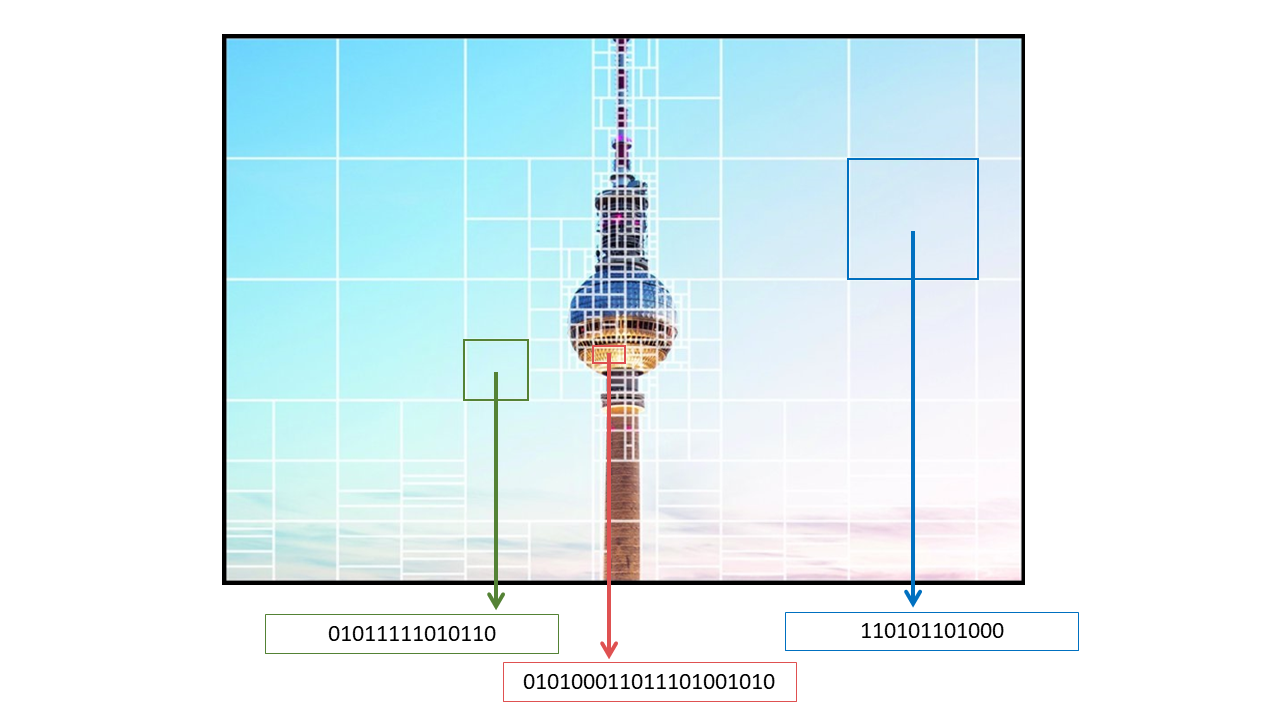
\includegraphics[width=0.35\textwidth]{comprclass.png}
%\captionsetup{labelformat=empty}
%\caption{Example for handwritten digits from MNIST.}
\end{figure}
\item Example: A typical image or video compression scheme partitions an image. 
Then, to each part, a collection of syntax elements is assigned and coded. Each syntax 
element can be interpreted as a class label $\mathbf{\rightarrow}$ Compression problem can be regarded as a collection of classification problems. 
\end{itemize}
\end{frame}


\subsection{Probabilistic framework}
\begin{frame}{Probabilstic framework both in ML and data compression}
\bit
\item Typical framework for many ML problems and for many compression problems is probabilistic.
\item Example: Prediction problems. 
\bit 
\item Machine learning problem: 
\bit
\item Given an observed variable $x$ , for a target variable $t$,  find a model for the conditional probabilty $p(t|x)$.
\item Finding a deterministic function, $t=f(x)$ is typically unrealistic for sufficiently complex problems.  
\eit
\item  Similar situation in compression:
\bit
\item Given already decoded information, in principle, any value for the current information is transmittable. 
\item However: Not every value is equally likely. This is exploited in entropy coding and in predictive coding. 
\eit
\eit
\item True probability distribution of the source is usually not known both in ML and compression problems.  
\item Rather: Either make some assumptions to study some model cases or work with empirical distributions, obtained from large data sets.
\eit
\end{frame}


\subsection{A concrete example: ML-perspective}
\begin{frame}{ML and compression. A concrete example. Dimensionality reduction (ML) and transform coding (compression)}
\uncover<2->{\STRUC{A problem in machine learning: }
\bit
\item Given a large set of data of high dimension.
\item Goal: Represent the data as accurately as possible in some lower dimensional space.  
\eit}
\uncover<2->{\STRUC{A basic algorithm: Principal component analysis: }
\bit 
\item Project data to the space generated by eigenvectors for the largest eigenvalues of the sample covariance matrix.  
\item If $N$ is the dimension of the data-space, PCA gives the best k-dimensional subspace approximation for each $k\leq N$. 
\item Generalizations like non-linear PCA, i.e. PCA in feature space, also exist. 
\eit
}
\end{frame}

\begin{frame}\frametitle{Example of a PCA}
Taken from Bishop, Pattern Recognition and Machine Learning 
\begin{itemize}
\item Consider a dataset that consists of a large collection of handwritten digits of the number $3$, taken from MNIST dataset.
\item Each data-sample of a handwritten digit is a grey-scale image with $28\times 28$ pixels. 
\item Thus: Data samples correspond to vectors $x_d\in \mathbb {R}^N$ for $N=748$. 
\end{itemize}
\begin{figure}
\centering

\includegraphics[width=0.95\textwidth]{number_3_MNIST.png}
\captionsetup{labelformat=empty}
\caption{Example for handwritten digits from MNIST.}
\end{figure}
\end{frame}

\begin{frame}{ Visualization of principal components} 
%\bit
%\item Mean and first principal components generate a low dimensional subspace in which the data can be represented with expected high accuracy.
%\eit
\begin{figure}
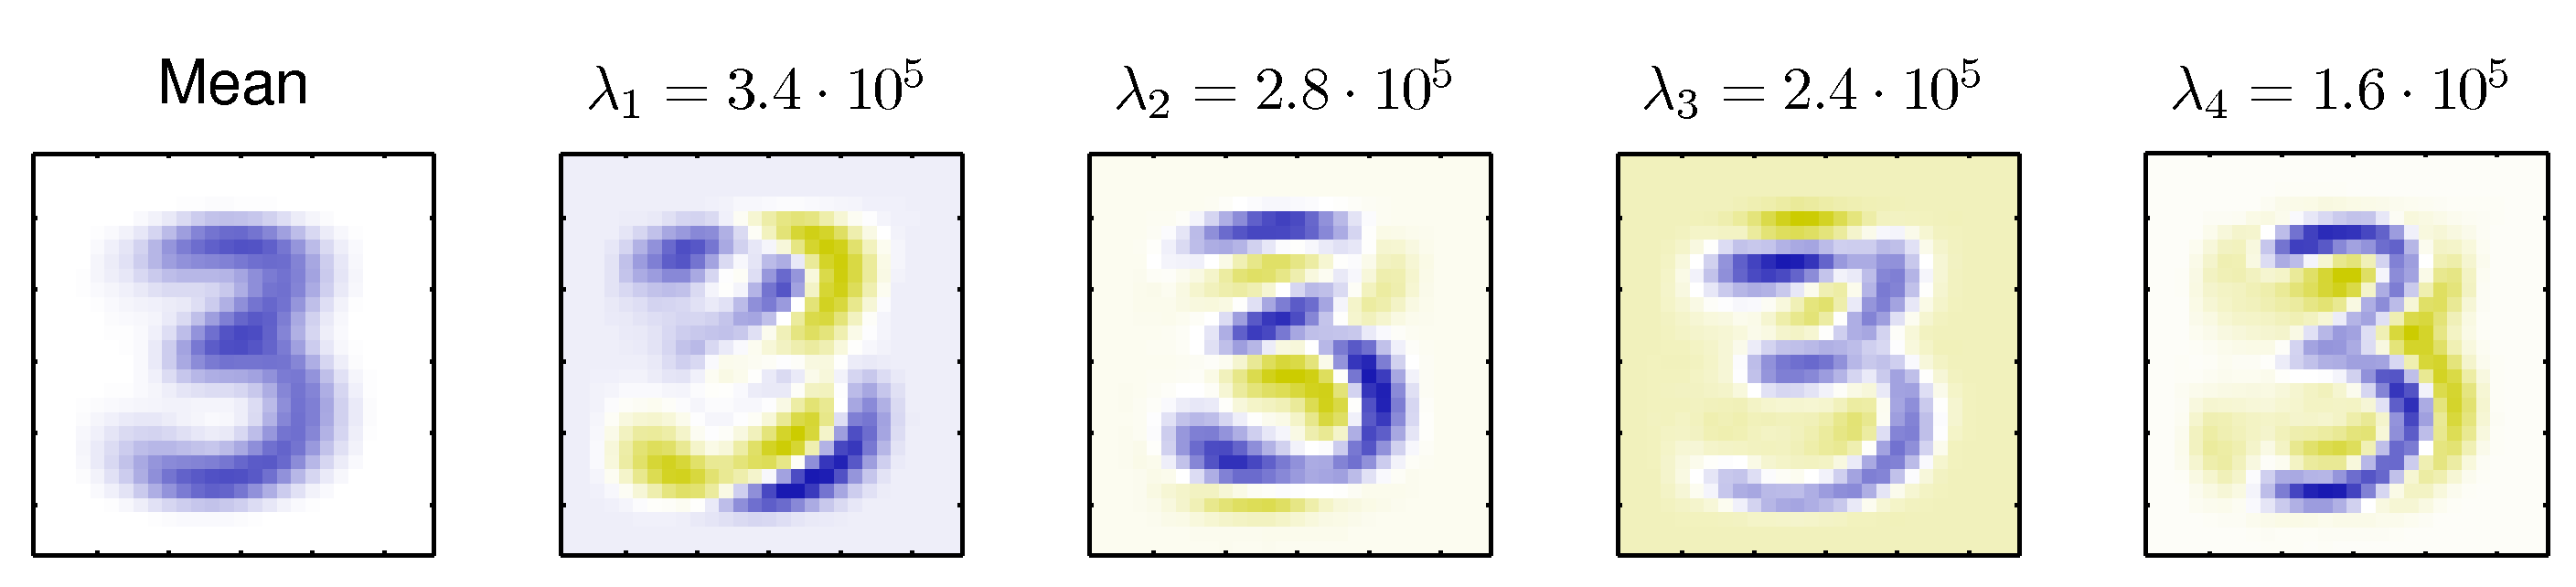
\includegraphics[width=.75\textwidth]{FigurePCA_1.png}
%\captionsetup{labelformat=empty}
%\caption{The mean (blue) and the first four principal components $v_1,\dots,v_4$ (yellow) of the handwritten digits of the number 3. These are the eigenvectors for the four largest eigenvalues $\lambda_1\geq\cdots\geq \lambda_4$ of the emprical covariance matrix of the MNIST-dataset for the digit 3. }
\end{figure}
\bit
\item The mean (blue) and the first four principal components $v_1,\dots,v_4$ (yellow) of the handwritten digits of the number 3.
\item The displayed principal components are the eigenvectors for the four largest eigenvalues $\lambda_1\geq\cdots\geq \lambda_4$ of the covariance matrix of the data-set.
\eit
\end{frame}

\begin{frame}{Visualization of energy compaction of PCA}
\begin{figure}
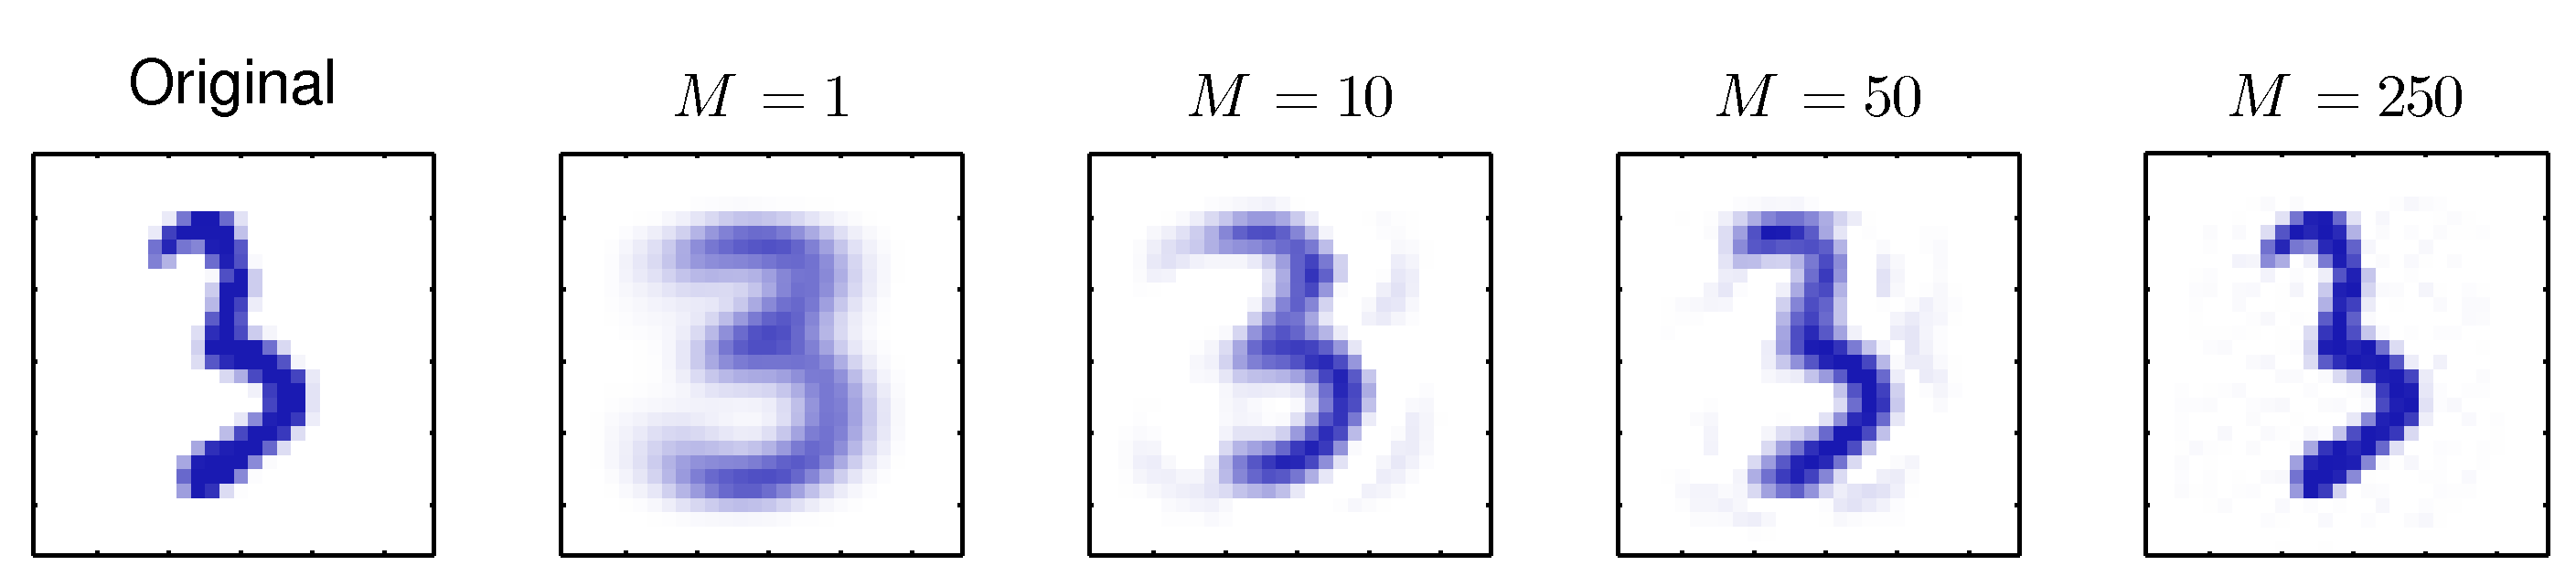
\includegraphics[width=.75\textwidth]{FigurePCA_2.png}
%\captionsetup{labelformat=empty}
%\caption{Example of an original handwritten digit (left), and its representation by using only a subset $v_1,\dots,v_M$ of the principal components and the mean of the data.
%It can be seen that $M\ll 748$ principal components suffice to represent the given example on the left accurately.
%}
\end{figure}
\bit
\item Example of an original handwritten digit (left), and its representation by using only a subset $v_1,\dots,v_M$ of the principal components and the mean of the data.
\item It can be seen that $M\ll 748$ principal components suffice to represent the given example on the left accurately.
\eit
\end{frame} 

\subsection{A concrete example:  Data compression perspective}
\begin{frame} {Dimensionality reduction and transform coding: Data compression perspective}
\uncover<2->{\STRUC{A problem in source coding:}
\bit
\item Projection data to be transmitted to some lower dimensional space.
\item Transmit only the information that is left after the projection.  
\item  Approach has to be suitable for compression: 
\item[\iarrow]\textbf{Keep high sampel-wise fidelity while reducing the transmission rate.} 
\eit
}
\uncover<2->{\STRUC{Basic concept: Transform coding}
\bit
\item Applying PCA to the data seems to be a good choice. In some model cases, PCA is optimal.  
\item But: Transform should be signal-independent, `suitable for the whole set of natural images'. 
\item Will be shown: DCT-II can be seen as a signal-independent approximation of PCA. 
\item Transform coding with DCT-II is a cornerstone of many widely deployed image and video codecs:
\bit
\item JPEG
\item H. 264/AVC
\item H. 265/HEVC
\eit
\eit
}
\end{frame}

\begin{frame} {DCT-II basis functions}
\begin{figure}
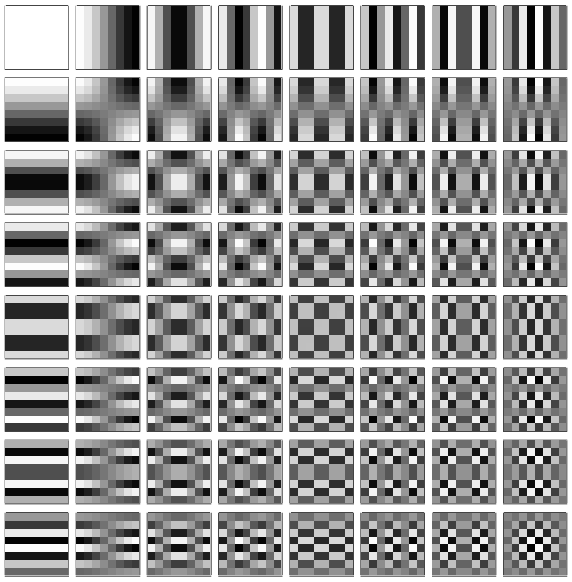
\includegraphics[width=.35\textwidth]{DCT8x8Basis.png}
%\captionsetup{labelformat=empty}
%\caption{Example of an original handwritten digit (left), and its representation by using only a subset $v_1,\dots,v_M$ of the principal components and the mean of the data.
%It can be seen that $M\ll 748$ principal components suffice to represent the given example on the left accurately.
%}
\end{figure}
\bit
\item The 64 basis functions of the Discrete Cosine Transform (DCT)-II transform on an $8x8$-block
\eit
\end{frame}

%\begin{frame} {Energy compaction of the DCT}
%\begin{figure}
%     \centering
%     \begin{subfigure}[b]{0.3\textwidth}
%         \centering
%         \includegraphics[width=1.25\textwidth]{HHI_Bild.jpg}         
%     \end{subfigure}
%     \quad\quad\quad
%          \begin{subfigure}[b]{0.3\textwidth}
%         \centering
%         \includegraphics[width=1.25\textwidth]{transformed.jpg}         
%     \end{subfigure}
%\end{figure}
%
%
%
%%\includegraphics[width=.35\textwidth]{HHI_Bild.jpg}
%%\captionsetup{labelformat=empty}
%%\caption{Example of an original handwritten digit (left), and its representation by using only a subset $v_1,\dots,v_M$ of the principal components and the mean of the data.
%%It can be seen that $M\ll 748$ principal components suffice to represent the given example on the left accurately.
%%}
%
%
%
%\bit
%\item Original image (left) and image represented using only ... percent of the  64 basis functions of the $8x8$-DCT-II. 
%\item Images is divided in $8x8$-blocks to apply the $8x8$-DCT-II. 
%\eit
%\end{frame}

\begin{frame}{Energy compaction of the DCT}
\begin{figure}
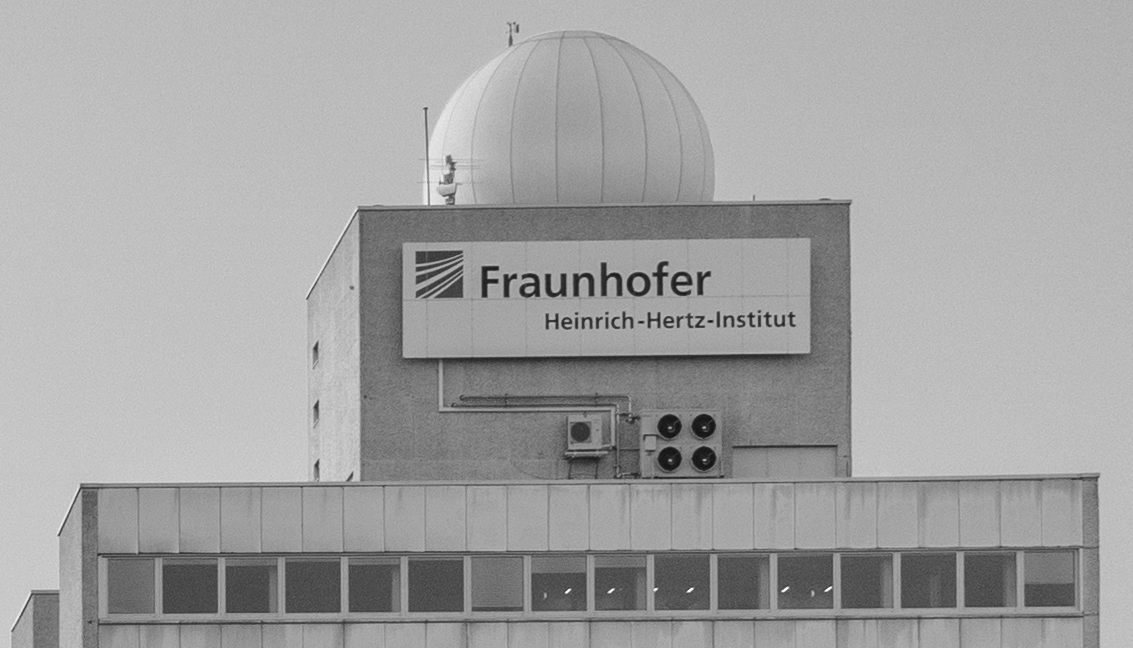
\includegraphics[width=0.70\textwidth]{HHI_gray_ausschnitt.png}
\captionsetup{labelformat=empty}
\caption{Original image.}
\end{figure}
\end{frame}

\begin{frame}{Energy compaction of the DCT}
\begin{figure}
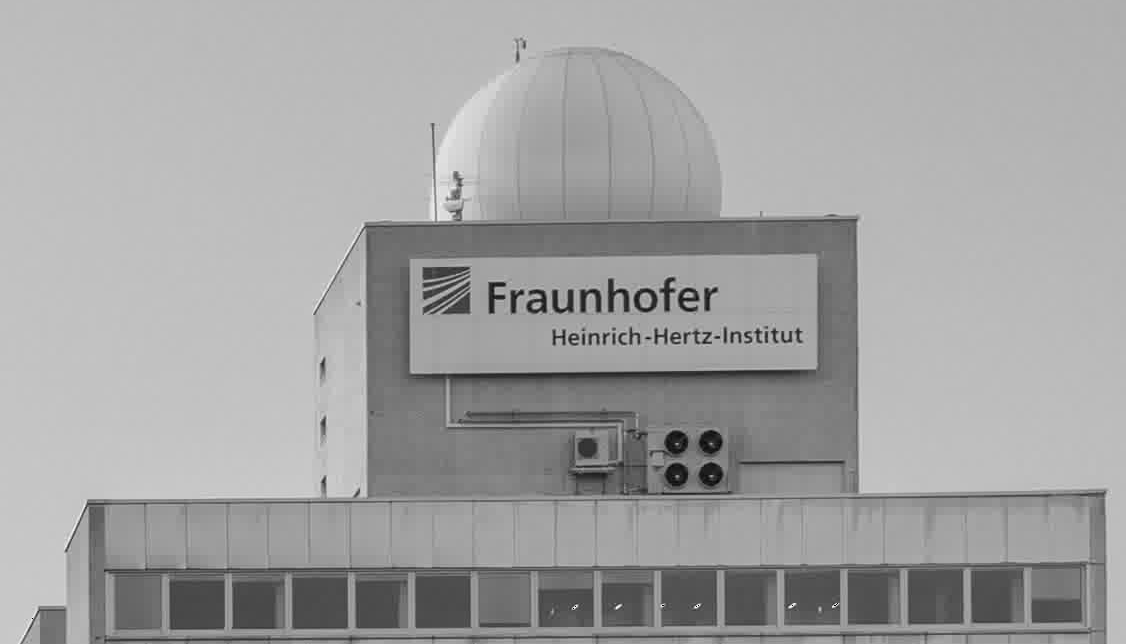
\includegraphics[width=0.70\textwidth]{HHI_gray_trafozero_ausschnitt.png}
\captionsetup{labelformat=empty}
\caption{Image represented using only $\sim 10\%$ percent of the  64 basis functions of the $8x8$-DCT-II on each block on average. Image is divided into $8x8$-blocks to apply the $8x8$-DCT-II. }
\end{figure}
\end{frame}



\subsection{Possible differences in objectives}
\begin{frame}{Distortion function of ML not always suitable for compression }
\begin{figure}
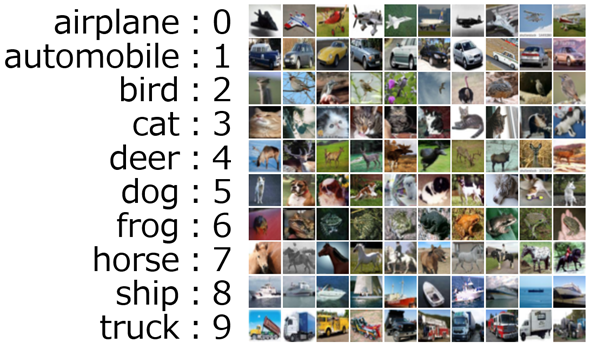
\includegraphics[width=.45\textwidth]{Cifar_2.png}
\end{figure}
\bit
\item Example of images from the CIFAR dataset. \\
\item Typical classification task in ML: Recognize the class $\rightarrow$ images in each row can be regarded as equal from this perspective.
\item However: Images in each row strongly deviate in terms of mean-squared error $\rightarrow$ images in each row not equal from compression perspective. 
\eit
\end{frame}

\begin{frame}{Distortion function of compression not always suitable for ML}
\begin{figure}
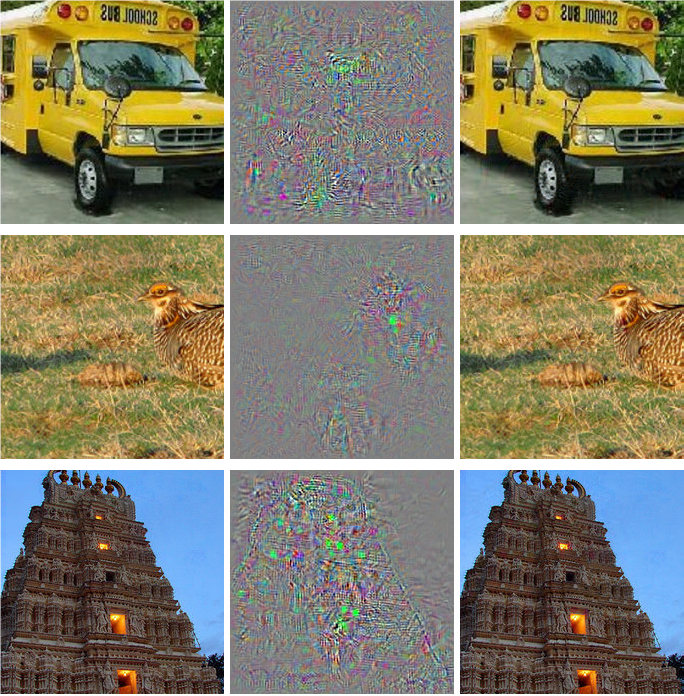
\includegraphics[width=.23\textwidth]{Adversarial.png}
%\captionsetup{labelformat=empty}
%\caption{Images in the left and right column have little deviation in terms of sample-wise mean-squared error $\longrightarrow$ similar 
%from a compression perspective. \\
%However: Standard CNN-based classifier AlexNet correctly classifies left column but misclassifies right column as ostrich $\longrightarrow$ not similar from a
%a machine-learning perspective.
%}
\end{figure}
\bit
\item Left and right columns have little deviation (middle column) in mean-squared error $\rightarrow$ similar 
from a compression perspective. \\
\item However: Standard CNN-based classifier AlexNet correctly classifies images in left column but misclassifies each image in right column as ostrich $\rightarrow$ not similar from a
a machine-learning resp. classification perspective.
\item Right column arises by so called adversarial attack to the AlexNet classifier. See: `Intriguing properties of neural networks', Szegedy et al., ICLR, 2014. 
\eit
\end{frame}
